% Multi-Objective Prompt Optimization: R-REBEL vs GRPO
%
% Draft scope (2026-09-08): algorithms + results only, per request. Intro is
% deliberately thin and related work is a stub -- see paper/README.md.
%
% Build:  make        (in paper/)   -- pdflatex x2 + bibtex
% Toolchain note: this cluster has pdflatex + bibtex but NO latexmk, and no
% algorithm2e/algpseudocode/pgfplots. The preamble therefore uses
% algorithm+algorithmic, and every figure is a pre-rendered PDF from
% analysis/paper_results.py rather than pgfplots.
\documentclass[11pt]{article}

\usepackage[letterpaper,margin=1in]{geometry}
\usepackage{amsmath,amssymb,bm}
\usepackage{booktabs}
\usepackage{graphicx}
\usepackage{subcaption}
\usepackage{microtype}
\usepackage{xcolor}
\usepackage{algorithm}
\usepackage{algorithmic}
\usepackage[numbers,sort&compress]{natbib}
\usepackage[colorlinks=true,linkcolor=blue!55!black,citecolor=blue!55!black,
            urlcolor=blue!55!black]{hyperref}

\graphicspath{{figures/}}

% ---- notation ------------------------------------------------------------
\newcommand{\pol}{\pi_\theta}
\newcommand{\polref}{\pi_{\mathrm{ref}}}
\newcommand{\lm}{p_{\mathrm{LM}}}
\newcommand{\lmb}{\lambda}
\newcommand{\Rlam}{r_{\lmb}}
\newcommand{\logratio}{\ell_\theta}
\newcommand{\Ggrp}{G}
\newcommand{\rrebel}{\mbox{R-REBEL}}          % prose (unbreakable)
\newcommand{\rrmath}{\text{R-REBEL}}          % math superscripts (scales)
% flags an open item; remove before submission
\newcommand{\todo}[1]{\textcolor{red!70!black}{[\textbf{TODO:} #1]}}

\title{Multi-Objective Prompt Optimization with a $\lambda$-Conditioned Policy:\\
       Robust Pairwise Regression Beats Group-Relative Policy Optimization}
\author{Aditya Deshmukh \and Lav R. Varshney}
\date{Draft --- \today}

\begin{document}
\maketitle

\begin{abstract}
We study prompt optimization for a multi-objective text task, where a single
policy must trace an entire tradeoff curve rather than reach one operating
point. A $\lmb$-conditioned policy emits a short discrete prompt that steers a
\emph{frozen} task language model; $\lmb$ indexes how tightly content
preservation is required, and sweeping it traces a content-versus-sentiment
curve. We train this policy with \rrebel{}, a family of objectives that
regresses the $\beta$-scaled log-ratio difference of two sampled prompts onto
their reward difference under a robust discrepancy, and we compare it against
GRPO on a Yelp negative-to-positive rewriting benchmark. Across five arms and
three seeds trained for $12{,}000$ steps, the best \rrebel{} variants reach
$39.3$ mean reward against $33.4$ for the strongest GRPO arm --- a $6.0$-point
gap, six times the $1$-point evaluation noise floor, with \emph{every} \rrebel{}
seed above \emph{every} GRPO seed. The GRPO baseline was both debugged (a
reference-anchor defect worth $+4.1$ points) and tuned (an entropy bonus worth a
further $+1.8$) before this comparison was drawn, so the remaining gap is not an
artifact of an under-configured baseline.
\end{abstract}

\section{Introduction}
\label{sec:intro}

Most reinforcement learning for language models optimizes a single scalar
reward and returns a single policy. Many real objectives are not like that. In
attribute-controlled rewriting, a system must satisfy two objectives in tension
--- change the attribute, preserve the meaning --- and the useful artifact is
not one operating point but the whole tradeoff curve, so that a downstream user
can choose where on it to sit. Training one policy per point is wasteful and
gives no guarantee that the points are mutually consistent.

We study this in the prompt-optimization setting, where the trainable object is
a short discrete prompt that steers a \emph{frozen} task language model. Our
policy is conditioned on a scalar $\lmb$ that indexes how tightly content
preservation is required, so a single trained policy traces the entire
content-versus-sentiment curve by varying its conditioning input at test time.
This makes exploration unusually load-bearing: a policy that collapses onto one
prompt is not merely suboptimal, it becomes $\lmb$-independent and collapses the
curve to a point.

That observation motivates the algorithm we study. GRPO, the default choice for
this kind of problem, estimates a group-relative advantage and ascends it inside
a clipped trust region. But in a pipeline that takes one gradient update per
batch of rollouts --- as prompt optimization naturally does, because rollouts
are expensive and the policy is small --- the importance ratio is identically
one and the clip is provably inert, leaving the KL penalty as the objective's
only regularizer, and leaving its unconstrained optimum a deterministic policy.
\rrebel{} instead treats improvement as regression: it fits the $\beta$-scaled
log-ratio difference of two sampled prompts to their observed reward difference,
under a \emph{robust} discrepancy chosen because those reward differences are
noisy Monte Carlo estimates. Its fixed point is a tempered softmax --- a
distribution, not a point mass --- so exploration is a property of the objective
rather than a penalty added to it.

\paragraph{Contributions.}
\begin{itemize}\itemsep2pt
  \item A $\lmb$-conditioned prompt policy for multi-objective controlled
        rewriting, trained against a constrained reward in which $\lmb$ sets a
        content floor (Section~\ref{sec:setup}).
  \item \rrebel{}, a family of robust pairwise reward-difference regression
        objectives, and an analysis of why GRPO's trust region is inert in the
        single-update regime while \rrebel{}'s fixed point resists collapse
        (Section~\ref{sec:algos}).
  \item An empirical comparison over five arms and three seeds at $12{,}000$
        steps in which the best \rrebel{} variants reach $39.3$ mean reward
        against $33.4$ for the strongest GRPO arm, with every \rrebel{} seed
        above every GRPO seed --- and in which the GRPO baseline was first
        debugged ($+4.1$ points) and then tuned ($+1.8$ points), so the
        remaining gap cannot be attributed to an under-configured baseline
        (Section~\ref{sec:results}).
\end{itemize}

\section{Problem setup}
\label{sec:setup}

\paragraph{Prompted style transfer with a frozen task model.}
Let $x$ be a source sentence with an undesired attribute (here, a negative Yelp
review). A policy $\pol(\cdot \mid \lmb)$ emits a short discrete
\emph{prompt} $z = (z_1,\dots,z_L)$ of fixed length $L=5$ tokens. The prompt is
inserted into a fixed template together with the source,
\begin{equation}
  \texttt{template}(z, x) \;=\; \texttt{\{z\}\ "\{x\}"\ "} ,
\end{equation}
and a \emph{frozen}, inference-only task language model $\lm$ samples a
rewrite $y \sim \lm(\cdot \mid \texttt{template}(z,x))$. Only $\theta$ is
trained; $\lm$ receives no gradient. This is the prompt-optimization regime: the
action space is the discrete prompt, and the environment --- the task model plus
the scorers --- is a black box.

\paragraph{Two objectives.}
Each rewrite is scored on two axes, both on a $0$--$100$ scale:
\begin{itemize}\itemsep2pt
  \item \emph{content} $c(x,y) \in [0,100]$, a BERTScore-style similarity
        between the rewrite and its source, measuring how much of the original
        meaning survives;
  \item \emph{sentiment} $s(y) \in [0,100]$, the probability assigned to the
        target attribute by a fine-tuned BERT classifier.
\end{itemize}
The two are in genuine tension: copying $x$ verbatim maximizes $c$ and leaves
$s$ at the source value, while emitting a generic positive sentence maximizes
$s$ and destroys $c$.

\paragraph{A $\lmb$-indexed \emph{constrained} reward.}
Rather than a linear scalarization, the objectives are combined as a
constraint. For $\lmb \in [0,1]$, define
\begin{equation}
  \Rlam(z,x) \;=\;
  \begin{cases}
    s(y), & c(x,y) \;\ge\; 100\lmb, \\[2pt]
    0.01\,\bigl(c(x,y) - 100\lmb\bigr), & \text{otherwise,}
  \end{cases}
  \label{eq:reward}
\end{equation}
so $\lmb$ sets a \emph{content floor} at $100\lmb$: reward equals the sentiment
score wherever the floor is met, and otherwise degrades to a small negative
penalty proportional to the shortfall. Sweeping $\lmb$ from $0$ (no content
requirement --- pure sentiment) to $1$ (near-verbatim content required) traces
the tradeoff curve. The penalty branch is scaled by $0.01$ so that violation is
weakly informative rather than a flat rejection, which keeps the objective
differentiable-in-expectation and gives the policy a gradient to climb back
into the feasible region.

Because $\lm$ is stochastic, the reward used for learning is a Monte Carlo
average over $N = 50$ task-model samples per (prompt, source) pair,
\begin{equation}
  \hat{r}_{\lmb}(z,x) \;=\; \frac{1}{N}\sum_{n=1}^{N} \Rlam(z, x; y_n),
  \qquad y_n \sim \lm(\cdot \mid \texttt{template}(z,x)),
  \label{eq:mcreward}
\end{equation}
which is what every algorithm below consumes as its scalar reward.

\paragraph{Objective: one policy for the whole curve.}
During training $\lmb$ is drawn afresh per source, $\lmb \sim \mathcal{U}[0,1]$,
and supplied to the policy as a conditioning input. A single set of parameters
$\theta$ must therefore serve every point on the curve, so that at test time the
frontier is traced by varying the conditioning input rather than by retraining:
\begin{equation}
  \max_{\theta}\;
  \mathbb{E}_{\lmb \sim \mathcal{U}[0,1]}\;
  \mathbb{E}_{x}\;
  \mathbb{E}_{z \sim \pol(\cdot \mid \lmb)}\bigl[\hat{r}_{\lmb}(z,x)\bigr].
  \label{eq:objective}
\end{equation}
This conditioning is what makes the problem multi-objective rather than a set of
independent single-objective runs, and it is the reason entropy collapse is
especially damaging here: a policy that collapses onto one prompt becomes
$\lmb$-independent and degenerates to a single point instead of a curve.

\section{Algorithms}
\label{sec:algos}

Both algorithms share the same outer loop, the same rollout mechanics, and the
same reward. For each of the $B=15$ sources in a batch, a fresh
$\lmb \sim \mathcal{U}[0,1]$ is drawn and $\Ggrp = 16$ prompts are sampled
i.i.d.\ from $\pol(\cdot \mid \lmb)$, forming a \emph{group} that shares a
source and a $\lmb$. Each prompt's reward $r_i = \hat{r}_{\lmb}(z_i, x)$ is the
Monte Carlo average of Eq.~\eqref{eq:mcreward}. The algorithms differ only in
how a group of $(z_i, r_i)$ pairs becomes a loss. Throughout, the policy
log-probability of a prompt is the token sum
\begin{equation}
  \log \pol(z \mid \lmb) \;=\; \sum_{t=1}^{L} \log \pol(z_t \mid z_{<t}, \lmb),
\end{equation}
and one crucial implementation fact holds for both methods: \textbf{exactly one
gradient update is taken per rollout}. There is no inner epoch loop.

\subsection{Baseline: GRPO}
\label{sec:grpo}

GRPO replaces a learned critic with a group-relative advantage. Within each
group, rewards are standardized,
\begin{equation}
  A_i \;=\; \frac{r_i - \mathrm{mean}(r_{1:\Ggrp})}
                 {\mathrm{std}(r_{1:\Ggrp}) + \varepsilon},
  \qquad \varepsilon = 10^{-8},
  \label{eq:grpo-adv}
\end{equation}
and the policy maximizes a clipped surrogate against a KL penalty toward a
reference policy $\polref$. With $\rho_{i,t}$ the per-token importance ratio,
the implemented loss is
\begin{equation}
  \mathcal{L}^{\mathrm{GRPO}}(\theta)
  = -\frac{1}{\Ggrp L}\sum_{i=1}^{\Ggrp}\sum_{t=1}^{L}
      \min\!\bigl(\rho_{i,t} A_i,\;
        \mathrm{clip}(\rho_{i,t}, 1-\epsilon_c, 1+\epsilon_c) A_i \bigr)
    \;+\; \beta_{\mathrm{KL}}\, \widehat{\mathrm{KL}}_{i,t},
  \label{eq:grpo}
\end{equation}
with $\epsilon_c = 0.2$ and the standard $k_3$ estimator, written in terms of
$u_{i,t} = \log \polref(z_{i,t}) - \log \pol(z_{i,t})$,
\begin{equation}
  \widehat{\mathrm{KL}}_{i,t} \;=\; e^{u_{i,t}} - u_{i,t} - 1 \;\ge\; 0 .
  \label{eq:k3}
\end{equation}
Because prompts have fixed length $L$, the token mean in Eq.~\eqref{eq:grpo}
carries no length bias, so the length-normalization critique levelled at GRPO by
Dr.\ GRPO does not apply in this setting. An optional entropy bonus
$-\,\alpha_H H(\pol)$ may be added; it is off in the plain baseline.

\paragraph{The clip is provably inert here, and this matters.}
With a single update per rollout, the behaviour policy \emph{is} the current
policy, so $\rho_{i,t} \equiv 1$ identically --- both in value and, since $1$
lies strictly inside $[1-\epsilon_c, 1+\epsilon_c]$, in gradient. The two
branches of the $\min$ therefore coincide, and Eq.~\eqref{eq:grpo} reduces to
REINFORCE with a group-normalized advantage plus a KL penalty:
\begin{equation}
  \nabla_\theta \mathcal{L}^{\mathrm{GRPO}}
  = -\frac{1}{\Ggrp L}\sum_{i,t} A_i \nabla_\theta \log \pol(z_{i,t})
    \;+\; \beta_{\mathrm{KL}} \nabla_\theta \widehat{\mathrm{KL}} .
\end{equation}
The consequence is structural rather than cosmetic: \textbf{the KL term is the
only thing regularizing this objective}. Its unconstrained optimum is a
deterministic policy --- put all mass on the group's best prompt --- so with the
trust region inactive, GRPO's fixed point in this pipeline is entropy collapse.
Implementations that run GRPO with $\beta_{\mathrm{KL}} = 0$ (TRL's default;
DAPO; Dr.\ GRPO) can do so because they take multiple epochs per rollout, which
keeps the clip live. This pipeline does not, so we set
$\beta_{\mathrm{KL}} = 0.04$, the canonical DeepSeekMath value.

\paragraph{The reference anchor must be long-lived.}
A KL penalty only regularizes if the anchor is stable. If $\polref$ is
re-copied from the live policy every $k$ steps, then each refresh sets both the
penalty and its gradient to zero, and for small $k$ the anchor never accumulates
restoring force --- the policy drifts arbitrarily far from initialization while
staying within $\sim\!1\%$ of a reference that chases it. We therefore
\emph{pin} the anchor for the entire run ($k = 0$: no re-anchoring), matching
TRL's \texttt{sync\_ref\_model=False} default, verl's and OpenRLHF's frozen
reference, and DeepSeekMath's once-per-outer-iteration re-anchoring.
Section~\ref{sec:baseline-defense} reports what this fix is worth empirically.

\begin{algorithm}[t]
\caption{GRPO as implemented (one update per rollout, pinned KL anchor)}
\label{alg:grpo}
\begin{algorithmic}[1]
\STATE \textbf{input} policy $\pol$, group size $\Ggrp$, KL weight $\beta_{\mathrm{KL}}$, clip $\epsilon_c$
\STATE $\polref \leftarrow \pol$ \COMMENT{pinned once; never re-anchored}
\FOR{step $= 1$ \TO $T$}
  \STATE draw a batch of sources $x^{(1..B)}$ and $\lmb^{(b)} \sim \mathcal{U}[0,1]$
  \FOR{each source $b$}
    \STATE sample $z_1,\dots,z_\Ggrp \sim \pol(\cdot \mid \lmb^{(b)})$
    \STATE $r_i \leftarrow \hat{r}_{\lmb^{(b)}}(z_i, x^{(b)})$ \COMMENT{avg.\ of $N=50$ frozen-task-LM samples}
    \STATE $A_i \leftarrow (r_i - \mathrm{mean}(r))/(\mathrm{std}(r) + \varepsilon)$
  \ENDFOR
  \STATE $\mathcal{L} \leftarrow$ Eq.~\eqref{eq:grpo} averaged over all groups and tokens
  \STATE one gradient step on $\theta$ \COMMENT{$\Rightarrow \rho \equiv 1$, clip inert}
\ENDFOR
\end{algorithmic}
\end{algorithm}

\subsection{\rrebel{}: robust pairwise reward-difference regression}
\label{sec:rrebel}

\rrebel{} discards the advantage-and-clip machinery entirely and treats policy
improvement as a \emph{regression} problem. Define the $\beta$-scaled log-ratio
of a prompt against a reference policy,
\begin{equation}
  \logratio(z) \;=\; \beta\Bigl(\log \pol(z \mid \lmb) - \log \polref(z \mid \lmb)\Bigr).
  \label{eq:logratio}
\end{equation}
For every \emph{unordered pair} $(i,j)$, $i<j$, within a group, \rrebel{} asks
that the model's log-ratio difference match the observed reward difference, and
penalizes the mismatch with a discrepancy $d$:
\begin{equation}
  \mathcal{L}^{\rrmath}(\theta)
  \;=\; \frac{2}{\Ggrp(\Ggrp-1)} \sum_{i<j}
        d\Bigl(
          \underbrace{\logratio(z_i) - \logratio(z_j)}_{\text{model}}
          \;-\;
          \underbrace{(\tilde{r}_i - \tilde{r}_j)}_{\text{target}}
        \Bigr),
  \label{eq:rrebel}
\end{equation}
where $\tilde{r}$ is the preprocessed reward described below. Taking
$d(\cdot) = (\cdot)^2$ recovers REBEL, whose least-squares fixed point is the
tempered softmax
\begin{equation}
  \pi^\star(z) \;\propto\; \polref(z)\,\exp\!\bigl(r(z)/\beta\bigr).
  \label{eq:fixedpoint}
\end{equation}
This is the structural difference from GRPO, and the paper's central mechanistic
claim: \textbf{\rrebel{}'s optimum is a distribution, not a point mass.}
Exploration does not have to be bolted on by a KL penalty or an entropy bonus,
because a policy that collapses cannot satisfy Eq.~\eqref{eq:rrebel} --- a
deterministic policy makes every log-ratio difference infinite while the reward
differences stay finite and bounded. Since a $\lmb$-conditioned policy must
serve the entire curve, this matters more here than in single-objective RLHF: a
collapsed policy is not merely suboptimal, it is $\lmb$-independent and yields a
point instead of a frontier.

\paragraph{Robust discrepancies.}
The \emph{R} in \rrebel{} is the replacement of the squared loss by a robust
$d$. The motivation is that $\tilde{r}_i - \tilde{r}_j$ is a Monte Carlo
estimate: with $N=50$ stochastic task-model samples per prompt, a heavy right
tail in the sentiment classifier produces occasional large, spurious reward
differences, and under a squared loss a single such pair dominates the group's
gradient. We consider
\begin{equation}
  d(e) \in \Bigl\{\, e^2,\quad |e|,\quad
    \mathrm{Huber}_\delta(e),\quad
    \log\bigl(1 + \tfrac{e^2}{2c^2}\bigr) \,\Bigr\}
\end{equation}
--- squared ($\ell_2$, i.e.\ REBEL), absolute ($\ell_1$),
Huber with $\delta = 1$, and Cauchy with $c^2 = 1/2$ --- whose influence
functions are respectively unbounded, bounded, bounded, and redescending.

\paragraph{Reward preprocessing, and why it is scale-fair.}
Rewards are scaled by a constant and a $\lmb$-dependent factor, and then
optionally standardized within the group:
\begin{equation}
  \tilde{r}_i \;=\; \frac{\kappa\, g(\lmb)\, r_i}
                         {\mathrm{std}(\kappa g(\lmb) r_{1:\Ggrp}) + \varepsilon},
  \qquad \kappa = 0.1, \quad g(\lmb) = 2.2111 \cdot 10^{\lmb} - 2.1111 .
  \label{eq:rewardprep}
\end{equation}
The group standardization in the denominator \emph{exactly cancels} any positive
per-group scale, so for every \rrebel{} variant reported in this paper (all of
which use it) the constants $\kappa$ and $g(\lmb)$ have no effect on the
gradient. This is a deliberate fairness property rather than an accident: GRPO's
advantage normalization in Eq.~\eqref{eq:grpo-adv} cancels reward scale in the
same way, so neither family can benefit from a tuned reward scale that the other
lacks. Both families therefore regress or ascend on a scale-normalized target.

\paragraph{Reference policy.}
Unlike GRPO's pinned anchor, \rrebel{}'s $\polref$ is refreshed every
$150$ steps. This is not a hyperparameter choice but part of REBEL's
construction: Eq.~\eqref{eq:rrebel} regresses the log-ratio against reward
differences measured under the \emph{recent} policy, so the reference must lag
by a bounded amount. The asymmetry with GRPO is intentional and is exactly the
distinction that the earlier defect blurred (Section~\ref{sec:baseline-defense}).

\paragraph{Variants evaluated.}
We report three: $\ell_1$-std ($d = |\cdot|$, group standardization),
Huber-std ($d = \mathrm{Huber}_1$, group standardization), and
$\ell_1$-ent ($\ell_1$-std plus an entropy bonus $-\alpha_H H(\pol)$,
$\alpha_H = 0.01$). Plain $\ell_2$ (REBEL) was dropped after ranking fourth and
proving seed-unstable in an earlier campaign.

\begin{algorithm}[t]
\caption{\rrebel{} (robust pairwise reward-difference regression)}
\label{alg:rrebel}
\begin{algorithmic}[1]
\STATE \textbf{input} policy $\pol$, group size $\Ggrp$, scale $\beta$, discrepancy $d$, ref lag $K = 150$
\STATE $\polref \leftarrow \pol$
\FOR{step $= 1$ \TO $T$}
  \IF{step $\bmod\ K = 0$}
    \STATE $\polref \leftarrow \pol$ \COMMENT{bounded lag, required by the construction}
  \ENDIF
  \STATE draw sources $x^{(1..B)}$ and $\lmb^{(b)} \sim \mathcal{U}[0,1]$
  \FOR{each source $b$}
    \STATE sample $z_1,\dots,z_\Ggrp \sim \pol(\cdot \mid \lmb^{(b)})$
    \STATE $r_i \leftarrow \hat{r}_{\lmb^{(b)}}(z_i, x^{(b)})$; standardize to $\tilde{r}_i$ by Eq.~\eqref{eq:rewardprep}
    \STATE $\logratio(z_i) \leftarrow \beta(\log \pol(z_i) - \log \polref(z_i))$
  \ENDFOR
  \STATE $\mathcal{L} \leftarrow$ Eq.~\eqref{eq:rrebel} over all $\binom{\Ggrp}{2}$ within-group pairs
  \STATE one gradient step on $\theta$
\ENDFOR
\end{algorithmic}
\end{algorithm}

\section{Experimental setup}
\label{sec:setup-exp}

\paragraph{Task and data.}
Yelp sentiment transfer in the negative-to-positive direction
(\texttt{direction} $= 0\!\to\!1$). Content is measured by BERTScore against
the source; sentiment by a \texttt{bert-base-uncased} classifier fine-tuned on
Yelp.

\paragraph{Models.}
The policy is a \texttt{distilgpt2} backbone with a trained MLP adaptor head
(hidden width $2048$) that emits a fixed-length $L=5$ token prompt, with a
$\lmb$-conditioning input supplied to the head. The head is initialized with
Xavier-uniform weights at gain $10^{-4}$, which drives its output logits to
zero, so \textbf{the initial prompt distribution is numerically uniform over
the full $50{,}257$-token vocabulary}: the measured policy entropy at step $0$
is $10.824904$ against $\ln 50257 = 10.824905$. This matters for GRPO and is
revisited in Section~\ref{sec:algos-caveat}. The task model is
\texttt{gpt2-xl}, \textbf{frozen} and inference-only in \texttt{bfloat16},
served through vLLM with top-$k=10$ sampling. Only the adaptor is trained.

\paragraph{Training.}
$12{,}000$ steps; batch of $B=15$ sources per step with $\Ggrp=16$ prompts per
source ($240$ scored prompt-source rows per step, each scored with $N=50$
task-model samples); Adam at learning rate $10^{-4}$ with gradient-norm
clipping at $10$; $\lmb \sim \mathcal{U}[0,1]$ redrawn per source per step.
\rrebel{} uses $\beta = 0.5$ and refreshes its reference every $150$ steps;
GRPO uses $\beta_{\mathrm{KL}} = 0.04$ with a pinned reference. Note the two
$\beta$s are not comparable quantities --- one is a regression scale in
Eq.~\eqref{eq:logratio}, the other a KL coefficient in Eq.~\eqref{eq:grpo}.

\paragraph{Arms and seeds.}
Five arms $\times$ three seeds $=15$ runs:
three \rrebel{} variants ($\ell_1$-std, Huber-std, $\ell_1$-ent) and two GRPO
arms (plain, and with an entropy bonus $\alpha_H = 0.01$). A sixth,
\emph{superseded} GRPO configuration --- the rolling reference anchor described
in Section~\ref{sec:grpo} --- is reported separately in
Section~\ref{sec:baseline-defense} as the pre-fix baseline.

\paragraph{Evaluation protocol, and a serious caveat about it.}
Every $500$ steps the policy is evaluated over the $\lmb$ grid
$\{0, 0.1, \dots, 0.9\}$. The headline metric is \emph{mean reward}: the reward
of Eq.~\eqref{eq:reward} averaged over the evaluation set and then over the ten
$\lmb$ values; content and sentiment are averaged the same way.

The caveat is that this in-training evaluation runs on the \textbf{development
split, capped at $10$ sentences} --- not on the $500$-sentence held-out test
split. The cap is a speed hack in the data loader, and the training entry point
passes the development set as the evaluation set. \textbf{Every number in
this paper is therefore a $10$-sentence development-set number}, and no run in
this campaign was ever evaluated on the test split. Two consequences we do not
paper over: the effect sizes below carry a much wider confidence interval than
three seeds would suggest, and the absolute values are not comparable to
published test-split results. Evaluation is noisy for a second reason as well ---
the frozen task model samples stochastically (\texttt{vllm\_seed} unset during
the campaign), and re-running a single evaluation moved its score by $1.1$
points --- so we treat $\mathbf{1.0}$ \textbf{point as a noise floor} and report
differences below it as ties rather than rankings. The $6$-point family gap is
well outside that floor; the sub-$2$-point gaps between variants are not
resolvable at $n=10$.
\todo{run the $500$-sentence test-split evaluation and report it as the primary
table. \texttt{slurm/eval\_v4.slurm} does exactly this (it drives
\texttt{run\_eval.py}, which uses the test split) for the regeneration
campaign; the v3 numbers cannot be upgraded because their checkpoints are gone.}

\paragraph{Compute.}
Each run occupies one GPU ($\ge\!40$\,GB, natively bf16 --- L40S, A40, A100 or
H100) at roughly $25$\,s/step, and is executed as a chain of $4$-hour scheduler
cycles that resume from the most recent checkpoint. Generation by the frozen
task model accounts for $97.6\%$ of step time; content and sentiment scoring
together account for $2.3\%$, and the policy update for under $0.4\%$.

\paragraph{Matched-step comparison.}
Because the arms were launched at different times and restarted different
numbers of times, we compare at a matched step rather than at wall-clock
completion. Step $11{,}500$ is the largest step at which \emph{all fifteen} runs
have an evaluation, and it is the point used for the headline table; results at
step $12{,}000$ are reported alongside it with their reduced seed counts stated
explicitly (Section~\ref{sec:provenance} explains why three runs lack a
$12{,}000$ evaluation).

\section{Results}
\label{sec:results}

\subsection{Headline comparison}

Table~\ref{tab:main} reports the matched-step comparison at step $11{,}500$,
where all fifteen runs are present.

\begin{table}[t]
\centering
\begin{tabular}{lrrrc}
\toprule
Algorithm & Reward & Content & Sentiment & Seeds \\
\midrule
R-REBEL ($\ell_1$-std) & 39.34 & 56.25 & 53.70 & 3/3 \\
R-REBEL (Huber-std) & 39.27 & 58.62 & 49.55 & 3/3 \\
R-REBEL ($\ell_1$-ent) & 37.49 & 58.17 & 48.15 & 3/3 \\
GRPO + entropy & 33.36 & 53.57 & 50.57 & 3/3 \\
GRPO & 30.19 & 55.92 & 43.03 & 3/3 \\
\bottomrule
\end{tabular}

\caption{Mean reward, content, and sentiment at matched step $11{,}500$ ---
the largest step at which every arm has all three seeds. Reward is averaged
over the evaluation set and then over the $\lmb$ grid $\{0,\dots,0.9\}$. All
quantities are on a $0$--$100$ scale. Note the evaluation set here is the
$10$-sentence development split, not the held-out test split
(Section~\ref{sec:setup-exp}).}
\label{tab:main}
\end{table}

Three observations, in decreasing order of robustness.

\paragraph{1. The family gap is large and unambiguous.}
The best \rrebel{} variant scores $39.34$ against $33.36$ for the best GRPO arm:
a gap of $\mathbf{5.98}$ points, or six times the $1.0$-point noise floor. The
separation survives at the level of individual runs, which is the strongest form
the claim can take: the \emph{worst} \rrebel{} seed ($36.82$) beats the
\emph{best} GRPO seed ($34.65$) by $2.16$ points. There is no overlap between
the two families' seed distributions, so the ordering does not depend on seed
selection or on averaging. Averaged over the second half of training
(steps $\ge 6000$), the same picture holds: $39.37$ and $39.44$ for
$\ell_1$-std and Huber-std versus $31.11$ and $33.17$ for the two GRPO arms.

\paragraph{2. The top two \rrebel{} variants are tied.}
$\ell_1$-std ($39.34$) and Huber-std ($39.27$) differ by $0.07$ points, far
inside the noise floor, and their per-seed ranges overlap almost completely
($39.0$--$39.9$ versus $38.7$--$40.0$). We therefore report them as tied and
draw no conclusion about which robust discrepancy is preferable.
$\ell_1$-ent, at $37.49$, is a genuine $1.85$ points behind --- adding an
entropy bonus to $\ell_1$-std \emph{hurt}, which is consistent with the claim in
Section~\ref{sec:rrebel} that \rrebel{} does not need an explicit exploration
term because its fixed point is already a distribution.

\paragraph{3. GRPO's deficit is in sentiment, not content.}
The component columns of Table~\ref{tab:main} locate the failure.
Plain GRPO's content score ($55.92$) is competitive with $\ell_1$-std's
($56.25$), but its sentiment score is $43.03$ against $53.70$ --- a $10.7$-point
shortfall that accounts for essentially the entire reward gap. Adding an entropy
bonus moves GRPO's sentiment up to $50.57$ but at the cost of content, which
falls to $53.57$, the lowest of any arm. In other words the GRPO arms can
purchase one objective or the other but cannot hold both at once, which is
precisely the pathology a $\lmb$-conditioned policy must avoid.
Figure~\ref{fig:components} shows this as a training-time trajectory: the
content panels are tightly bunched across all five arms, while the sentiment
panel separates the families cleanly.

\begin{figure}[t]
\centering
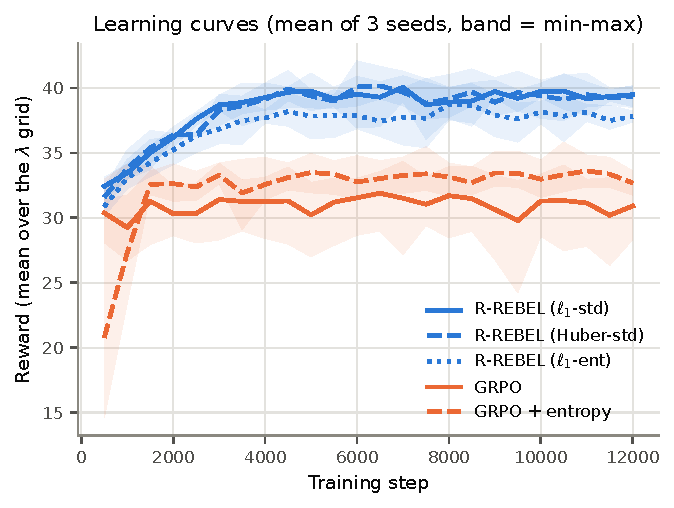
\includegraphics[width=0.82\textwidth]{learning_curves.pdf}
\caption{Mean reward against training step, averaged over three seeds, with the
band spanning the seed minimum to maximum. The two families separate by step
$\sim\!2000$ and never re-cross. Blue denotes \rrebel{} variants, orange the
GRPO arms.}
\label{fig:learning}
\end{figure}

\begin{figure}[t]
\centering
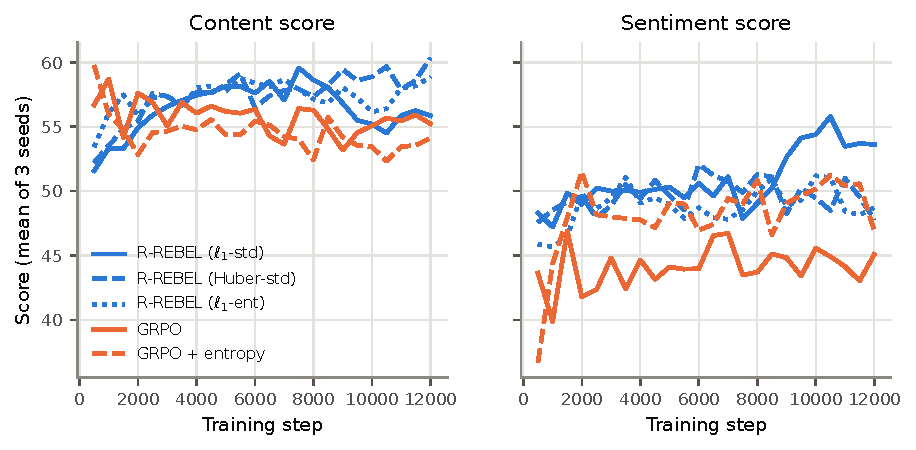
\includegraphics[width=\textwidth]{components.pdf}
\caption{The reward gap decomposed. Content (left) is comparable across all
arms; sentiment (right) is where plain GRPO falls away. Both panels share a
$y$-scale, so the difference in spread between them is directly comparable.}
\label{fig:components}
\end{figure}

\subsection{Learning dynamics}

Figure~\ref{fig:learning} shows that the outcome is not a late-training
artifact. All arms improve rapidly over the first $\sim\!1500$ steps; the two
families have separated by step $2000$ and never cross again. The \rrebel{}
variants climb to roughly $39$--$40$ and then plateau, whereas both GRPO arms
flatten early --- plain GRPO at $\sim\!31$ and GRPO-plus-entropy at $\sim\!33$
--- and stay flat for the remaining $10{,}000$ steps. The seed bands are also
informative: GRPO's band is markedly wider (its seeds at step $11{,}500$ span
$26.33$ to $34.65$, an $8.3$-point spread, versus $36.82$--$40.00$, a
$3.2$-point spread, across all nine \rrebel{} seeds), so the baseline is both
worse on average and less reliable.

\paragraph{Plain GRPO does not plateau --- it never learns at all.}
This distinction matters, and reading Figure~\ref{fig:learning} as ``GRPO
converges lower'' would be too generous to our own result. Measured from its
\emph{first} evaluation at step $500$ to step $11{,}500$, the plain GRPO arm
moves from $30.38$ to $30.19$: a change of $\mathbf{-0.18}$ points over
$11{,}000$ training steps, inside the noise floor and slightly negative. The
per-seed deltas are $+0.11$, $+1.09$ and $-1.75$. For comparison, over the same
interval \rrebel{} ($\ell_1$-std) gains $+6.74$, $+6.23$ and $+7.77$, and
GRPO-plus-entropy gains $+17.74$, $+3.23$ and $+16.77$. Two corroborating
diagnostics from the training logs: the logged KL sits at $9.824$ against the
$k_3$ estimator's analytic ceiling of $9.8249$ for a $50{,}257$-token
vocabulary --- attained only when the sampled token has probability $\approx 1$
--- and the count of distinct prompt tokens explored per training cycle has a
median of $5$, which for a $5$-token prompt means a single frozen,
$\lmb$-independent prompt.

So the plain GRPO number in Table~\ref{tab:main} is the score of a policy that
collapsed by step $500$ and never moved again. It is a \emph{diagnostic}, not a
converged baseline, and we do not present it as one: \textbf{the defensible GRPO
baseline in this paper is the GRPO-plus-entropy arm} at $33.36$, which does
learn. The headline comparison should be read against that arm --- a $5.98$-point
gap --- and plain GRPO read as evidence for the collapse mechanism of
Section~\ref{sec:grpo} rather than as a tuned competitor.
\todo{re-run plain GRPO with a competent (non-uniform) KL reference, per the
TODO in Section~\ref{sec:algos-caveat}, before claiming anything about GRPO's
ceiling as an algorithm.}

\subsection{The baseline was debugged and tuned, and still trails}
\label{sec:baseline-defense}

The most likely objection to a result of this shape is that the baseline was
misconfigured. It was, initially --- and fixing it is part of the result. We
report the full sequence in Figure~\ref{fig:baseline}, all at matched step
$4500$:

\begin{center}
\begin{tabular}{lrl}
\toprule
GRPO configuration & Mean reward & Change \\
\midrule
Rolling reference anchor (defective) & $27.16$ & --- \\
Pinned reference anchor (Section~\ref{sec:grpo}) & $31.30$ & $+4.14$ \\
\quad + entropy bonus $\alpha_H = 0.01$ & $33.10$ & $+1.80$ \\
\midrule
\rrebel{} (all variants, same step) & $39.26$ & $+6.16$ remaining \\
\bottomrule
\end{tabular}
\end{center}

The first row is the defect described in Section~\ref{sec:grpo}: the KL
reference was being re-copied from the live policy every $150$ steps, roughly
eighty times over a run, which zeroed the penalty and its gradient at every
refresh. Under that configuration GRPO's reward curve was flat from step $500$
onward, consistent with the entropy collapse that Section~\ref{sec:grpo}
predicts when the only regularizer is inert. Pinning the anchor is worth
$+4.14$ points. Giving GRPO the same entropy-bonus lever that $\ell_1$-ent has
is worth a further $+1.80$.

Both interventions behave as designed, which is evidence that they were
implemented correctly rather than merely tried. The entropy bonus in particular
starts \emph{worse} than plain GRPO and only overtakes it from step
$\sim\!1500$ onward --- the signature of a term that buys exploration at the
cost of early exploitation.

We must, however, retract one part of the defense. It would be convenient to say
that the two GRPO arms are two \emph{independent} chances for the baseline, so
that their agreeing on a $\sim\!31$--$33$ ceiling is strong evidence about GRPO
as an algorithm. That claim does not survive scrutiny. As
Section~\ref{sec:algos-caveat} shows, the pinned reference is the uniform
distribution, so plain GRPO already carries an implicit entropy coefficient of
$0.04$; the ``GRPO + entropy'' arm merely raises the total to $\approx\!0.05$.
The two arms are one configuration at two nearby settings of the same
anti-collapse lever, which is a natural explanation for their landing in the
same place, and it is \emph{not} independent corroboration. What the table above
does support is narrower but still real: a diagnosed defect was fixed and was
worth $+4.14$, an additional exploration lever was worth $+1.80$, and a
$6$-point gap to \rrebel{} remained after both.

\todo{the direct collapse evidence --- per-checkpoint counts of distinct emitted
prompts, which during the campaign read $2$--$19$ for defective GRPO against
$\sim\!97$ for \rrebel{} --- came from the per-$\lmb$ evaluation files and did
not survive the purge (Section~\ref{sec:provenance}). It is deliberately not
quoted as a measured result here. The surviving tracker metric
(\texttt{num\_tokens\_explored}) cannot substitute: it is a per-process
cumulative set that restarts on every $4$-hour resubmit, so its peak is
dominated by early-training exploration and does not measure steady-state
collapse. The rerun regenerates the original statistic; restore this paragraph's
numbers from it.}

\begin{figure}[t]
\centering
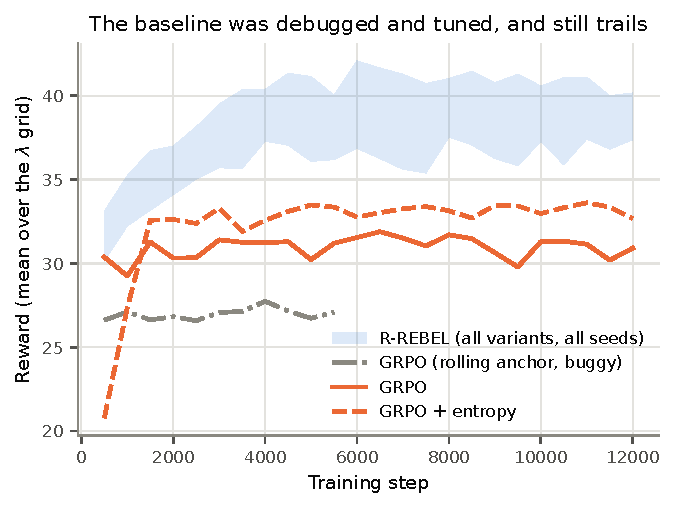
\includegraphics[width=0.82\textwidth]{baseline_debug.pdf}
\caption{The baseline-defense figure. The defective rolling-anchor GRPO (grey)
is flat at $\sim\!27$; pinning the anchor lifts it to $\sim\!31$ (solid orange);
adding an entropy bonus reaches $\sim\!33$ (dashed orange). The blue band is the
envelope over all three \rrebel{} variants and all their seeds. The rolling-anchor
runs were terminated once the defect was identified, hence their shorter extent.}
\label{fig:baseline}
\end{figure}

\subsection{The content--sentiment tradeoff curve}
\label{sec:tradeoff}

\begin{figure}[t]
\centering
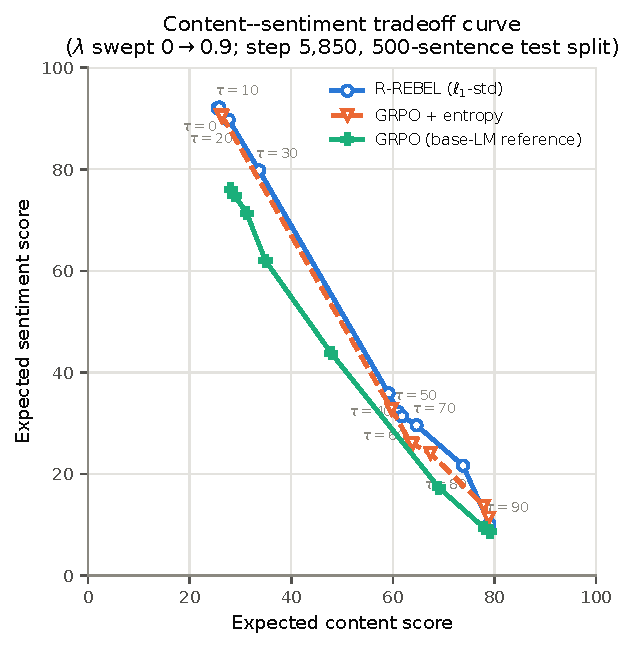
\includegraphics[width=0.6\textwidth]{tradeoff.pdf}
\caption{Content against sentiment at step $11{,}500$. Hollow markers are
individual seeds, filled markers each arm's mean. \textbf{These are
$\lmb$-averaged operating points, not a frontier}: each marker collapses the
whole $\lmb$ grid to one point. The per-$\lmb$ curve is pending
(Section~\ref{sec:provenance}). Even so, the \rrebel{} points sit up and to the
right of the GRPO points, i.e.\ better on both objectives simultaneously.}
\label{fig:tradeoff}
\end{figure}

The intended headline figure of this paper is the \emph{per-$\lmb$} curve: for
each arm, the locus of (content, sentiment) pairs obtained as $\lmb$ sweeps
$0 \to 0.9$, which shows not just that \rrebel{} scores higher but that it
commands a strictly better frontier. That figure cannot yet be drawn --- the
per-$\lmb$ evaluation arrays for the completed campaign were lost, as
Section~\ref{sec:provenance} details, and regenerating them requires
checkpoints, which are being retrained.

Figure~\ref{fig:tradeoff} therefore shows what the surviving data does support:
each run's single $\lmb$-averaged operating point. This is deliberately
\emph{not} presented as a frontier. It still carries a real claim --- the
\rrebel{} points lie up and to the right of the GRPO points, so \rrebel{}
dominates on both objectives at once rather than trading one for the other ---
but the shape of each arm's curve, and in particular whether GRPO's curve is
uniformly dominated or only dominated in the interior of the $\lmb$ range,
remains open until the rerun completes.
\todo{replace Figure~\ref{fig:tradeoff} with the true per-$\lmb$ frontier once
\texttt{slurm/eval\_v4.slurm} has produced
\texttt{results/v4/*/test/output*.json}; \texttt{analysis/paper\_results.py}
switches the figure over automatically and reports which version it drew.}


\subsection{Results at step 12{,}000}

\begin{table}[t]
\centering
\begin{tabular}{lrrrc}
\toprule
Algorithm & Reward & Content & Sentiment & Seeds \\
\midrule
R-REBEL ($\ell_1$-std) & 39.47 & 55.87 & 53.63 & 3/3 \\
R-REBEL (Huber-std) & 39.30 & 60.34 & 47.78 & 2/3 \\
R-REBEL ($\ell_1$-ent) & 37.80 & 58.88 & 48.72 & 2/3 \\
GRPO + entropy & 32.68 & 54.12 & 46.93 & 2/3 \\
GRPO & 30.91 & 55.24 & 45.09 & 3/3 \\
\bottomrule
\end{tabular}

\caption{The same quantities at step $12{,}000$, the nominal end of training.
Three runs have no evaluation at this step (Section~\ref{sec:provenance}), so
the seed counts differ by arm; the ordering and the size of the family gap are
unchanged from Table~\ref{tab:main}.}
\label{tab:12000}
\end{table}

Table~\ref{tab:12000} reports the nominal end of training. The conclusions do
not change: $\ell_1$-std ($39.47$) and Huber-std ($39.30$) remain tied within
noise, $\ell_1$-ent trails at $37.80$, and the GRPO arms sit at $32.68$ and
$30.91$. Because three runs are missing their $12{,}000$ evaluation, this table
is seed-unbalanced across arms and Table~\ref{tab:main} is the comparison we
rely on.

\subsection{Data provenance, and what is missing}
\label{sec:provenance}

Reporting this honestly requires a note on provenance, because it also bounds
what can currently be reproduced.

The campaign ran to completion, but its artifacts were subsequently destroyed:
the scratch filesystem holding all checkpoints and all per-$\lmb$ evaluation
files was purged, leaving zero checkpoints and zero evaluation files. Every
number in this paper was therefore recovered from the experiment tracker's
retained scalar history, by a reconstruction that is validated three ways per
run and refuses to emit data if any check fails: surviving true-step markers
must agree with the reconstructed step, the distinct-step count must be
consistent with the final step, and the reconstructed step grid must be
perfectly regular. All fifteen runs pass. Two consequences:

\begin{enumerate}\itemsep2pt
  \item \textbf{The per-$\lmb$ arrays are gone and are not recoverable from the
        tracker}, because the evaluation routine averages over the $\lmb$ grid
        \emph{before} logging. This is why Section~\ref{sec:tradeoff} shows
        operating points rather than a frontier. One seed per arm is being
        retrained specifically to regenerate them.
  \item \textbf{Three runs lack a step-$12{,}000$ evaluation.} Their final
        training cycle ran while the tracker was unreachable; the trainer's
        fallback keeps training without logging, so that cycle's evaluations
        were written only to the since-purged disk copies. This is why step
        $11{,}500$, not $12{,}000$, is the balanced comparison point.
\end{enumerate}

Two process changes follow, and are already in place: evaluation artifacts are
now copied off the purgeable filesystem after every training cycle, and the
recovery-and-validation script is committed alongside the exported data so that
every table in this paper can be regenerated from a single command.

\section{Limitations and threats to validity}
\label{sec:limitations}

We state these plainly, because several of them bound how strongly the headline
comparison can be read.

\paragraph{The reference policy is not a competent model.}
GRPO's pinned $\polref$ is the policy at initialization: an untrained MLP
adaptor head with a $-10$ logit bias, i.e.\ a near-uniform, high-entropy prompt
distribution --- not a supervised-fine-tuned model as in canonical RLHF
pipelines. Pinning such an anchor is a genuine departure from canonical GRPO.
It is anti-collapse, so it works in GRPO's favour here, but it also means the KL
term pulls toward high entropy rather than toward a good policy, and a GRPO run
starting from a competent reference might behave differently. This is the single
most important caveat on the comparison.

\paragraph{The tradeoff curve itself is not yet measured.}
As Sections~\ref{sec:tradeoff} and~\ref{sec:provenance} explain, the per-$\lmb$
frontier --- the figure this paper is nominally about --- is pending a rerun.
Everything reported here is $\lmb$-averaged. It remains possible that two arms
with similar average reward have differently-shaped curves, and the dominance
claim of Figure~\ref{fig:tradeoff} is about averaged operating points, not about
pointwise dominance across $\lmb$.

\paragraph{The rerun is single-seed.}
The regeneration campaign trains one seed per arm, not three. Its frontiers will
therefore be indicative rather than seed-averaged, and given GRPO's wide seed
spread ($26.3$--$34.7$ at step $11{,}500$) a single GRPO seed should not be read
as that arm's typical curve.

\paragraph{Evaluation noise and the number of seeds.}
Three seeds per arm and a $1.0$-point noise floor are enough to separate the
families ($6.0$ points) but not to rank variants within a family; we
consequently report the top two \rrebel{} variants as tied and draw no
conclusion between them. The noise floor is itself estimated from a single
repeated evaluation, so it is an order-of-magnitude figure rather than a
calibrated standard error.

\paragraph{The style classifier used at evaluation.}
The evaluation entry point requests the \emph{train}-split style classifier
rather than the test-split one. Since the same classifier scores every arm, this
cannot explain the family gap, but it does mean the absolute sentiment numbers
are not directly comparable to work that evaluates with the held-out
classifier.
\todo{confirm whether this is intentional; if not, re-evaluate with the
test-split classifier and update the absolute sentiment numbers. Arm ordering is
not at risk either way.}

\paragraph{Single task and single direction.}
All results are Yelp negative-to-positive with a \texttt{gpt2-xl} task model and
$5$-token prompts. We make no claim about other datasets, other transfer
directions, longer prompts, or larger task models. In particular, the inert-clip
argument of Section~\ref{sec:grpo} is a property of the single-update regime; a
pipeline that takes multiple epochs per rollout would keep GRPO's trust region
live and might close some of the gap.

\paragraph{Scope of this draft.}
Per its stated scope, this draft presents the algorithms and the results.
Related work is a stub, and there is no discussion or conclusion section yet.


\section{Related work}
\todo{stub --- out of scope for this draft, which covers algorithms and results
only. Needs: RL for discrete prompt optimization (RLPrompt and successors);
REBEL and regression-based policy optimization; GRPO and its variants (DAPO,
Dr.\ GRPO) with particular attention to the length-normalization and
KL-free-versus-clip discussion; multi-objective RLHF and reward-conditioned /
hypernetwork policies.}

% Bibliography is intentionally not wired up yet. The works named in prose
% (DeepSeekMath/GRPO, REBEL, DAPO, Dr. GRPO, TRL, verl, OpenRLHF, RLPrompt,
% BERTScore) are referenced by name only: entering them with invented keys,
% years or venues would be worse than leaving them uncited in a draft. Add real
% entries to refs.bib, then uncomment the two lines below.
\todo{populate refs.bib with verified entries and replace every by-name mention
in the prose with a \texttt{\textbackslash citep}. Works currently named
without citations: GRPO/DeepSeekMath, REBEL, DAPO, Dr.\ GRPO, TRL
GRPOTrainer, verl, OpenRLHF, BERTScore, and the RLPrompt line of discrete
prompt-optimization work.}
% \bibliographystyle{plainnat}
% \bibliography{refs}

\end{document}
